%%
%% This is file `sample-sigconf.tex',
%% generated with the docstrip utility.
%%
%% The original source files were:
%%
%% samples.dtx  (with options: `sigconf')
%% 
%% IMPORTANT NOTICE:
%% 
%% For the copyright see the source file.
%% 
%% Any modified versions of this file must be renamed
%% with new filenames distinct from sample-sigconf.tex.
%% 
%% For distribution of the original source see the terms
%% for copying and modification in the file samples.dtx.
%% 
%% This generated file may be distributed as long as the
%% original source files, as listed above, are part of the
%% same distribution. (The sources need not necessarily be
%% in the same archive or directory.)
%%

%% The first command in your LaTeX source must be the \documentclass command.
\documentclass[sigconf]{acmart} 
\settopmatter{printacmref=false}
\renewcommand\footnotetextcopyrightpermission[1]{} % removes footnote with conference information in first column


\usepackage{hyperref}  

%%
%% \BibTeX command to typeset BibTeX logo in the docs
\AtBeginDocument{%
  \providecommand\BibTeX{{%
    \normalfont B\kern-0.5em{\scshape i\kern-0.25em b}\kern-0.8em\TeX}}}
\setcopyright{none}
\hyphenation{De-zi-mal-tren-nung}
\renewcommand
\footnotetextcopyrightpermission[1]{}


\usepackage{xcolor}
\usepackage{placeins}

%%
%% Submission ID.
%% Use this when submitting an article to a sponsored event. You'll
%% receive a unique submission ID from the organizers
%% of the event, and this ID should be used as the parameter to this command.
%%\acmSubmissionID{123-A56-BU3}

%%
%% The majority of ACM publications use numbered citations and
%% references.  The command \citestyle{authoryear} switches to the
%% "author year" style.
%%
%% If you are preparing content for an event
%% sponsored by ACM SIGGRAPH, you must use the "author year" style of
%% citations and references.
%% Uncommenting
%% the next command will enable that style.
%%\citestyle{acmauthoryear}

%%
%% end of the preamble, start of the body of the document source.
\begin{document}\setlength\emergencystretch{1.5em}

%%
%% The "title" command has an optional parameter,
%% allowing the author to define a "short title" to be used in page headers.
\title{Dokumentation ITIL - Qualitätssicherungsteam}

%%
%% The "author" command and its associated commands are used to define
%% the authors and their affiliations.
%% Of note is the shared affiliation of the first two authors, and the
%% "authornote" and "authornotemark" commands
%% used to denote shared contribution to the research.

\author{Lara Krautmacher}
\email{lara.krautmacher@student.reutlingen-university.de}
\affiliation{%
  \city{Matrikelnummer: 801849}
  \institution{\\Informatik: IT-Management}
  \streetaddress{Alteburgstraße 150}
  \city{72762 Reutlingen}
  \state{Baden-Württemberg}
  \country{Deutschland}  
}
\author{René Wiskow}
\email{rené.wiskow@student.reutlingen-university.de}
\affiliation{%
  \city{Matrikelnummer: 801861}
  \institution{\\Informatik: IT-Management}
  \streetaddress{Alteburgstraße 150}
  \city{72762 Reutlingen}
  \state{Baden-Württemberg}
  \country{Deutschland}
}



\author{Elena Kirsch}
\email{elena.kirsch@student.reutlingen-university.de}
\affiliation{%
  \city{Matrikelnummer: 763207}
  \institution{\\Informatik: IT-Management}
  \streetaddress{Alteburgstraße 150}
  \city{72762 Reutlingen}
  \state{Baden-Württemberg}
  \country{Deutschland}
}


%%
%% By default, the full list of authors will be used in the page
%% headers. Often, this list is too long, and will overlap
%% other information printed in the page headers. This command allows
%% the author to define a more concise list
%% of authors' names for this purpose.


%%
%% The abstract is a short summary of the work to be presented in the
%% article.
\begin{abstract}
Qualitätssicherung spielt eine zentrale Rolle in jedem Unternehmen.
Reibungslose Abläufe interner Prozesse sowie die Erfüllung
von Ansprüchen an ein Endprodukt werden durch sie
garantiert. Im Zuge dieser Seminararbeit wird
im Rahmen eines Planspiels evaluiert wie mithilfe der IT Infrastructure
Library die Organisation und Durchführung einer effizienten Qualitätssicherung
umgesetzt werden kann. Dazu wurde das fiktive Unternehmen
\textit{TopBlogAG}, bestehend aus fünf Arbeitsgruppen, gegründet, welches
als Zielsetzung die Erstellung einer Blogging-Platform hat. Die
Arbeitsgruppe Qualitätssicherung hat dazu verschiedene Teststrategien
sowie Schwachstellenanalysen durchgeführt. Durch die Definition
von Key Performance Indicators in der Service-Quality Policy
ist festgelegt, wann die Ziele des Qualitätssicherungsprozesses
erreicht sind. 
\end{abstract}

%%
%% The code below is generated by the tool at http://dl.acm.org/ccs.cfm.
%% Please copy and paste the code instead of the example below.
%%


%%
%% Keywords. The author(s) should pick words that accurately describe
%% the work being presented. Separate the keywords with commas.
\keywords{IT-Management, ITIL, Qualitätssicherung, Service Transition}

%% A "teaser" image appears between the author and affiliation
%% information and the body of the document, and typically spans the
%% page.
\settopmatter{printfolios=true}
%%
%% This command processes the author and affiliation and title
%% information and builds the first part of the formatted document.
\maketitle
\pagestyle{plain} % removes running headers

\section{Einleitung - Elena}
\label{sec:intro}
Unternehmen sind bestrebt ihre Prozesse, Produkte oder auch Dienstleistungen durch Frameworks und Zertifizierungen zu verbessern und deren Qualität stetig zu steigern. 
Die Qualität von Produkten ist entscheidend wie gut sich ein Unternehmen in dem jeweiligen Markt etablieren kann. Im allgemeinen Sprachgebrauch steht das Wort \textit{Qualität} für die Beschaffenheit oder Eigenschaft einer Sache oder Person\footnote{https://www.duden.de/rechtschreibung/Qualitaet, Zugriff: 12.06.2021}. In der Wirtschaft bezeichnet Qualität den Wert oder die Güte einer Sach- oder Dienstleistung aus Sicht des Anwenders/der Anwenderin\footnote{http://wirtschaftslexikon24.com/d/qualitaet/qualitaet.htm, Zugriff: 12.06.2021}. Die ISO 9000:2015 beschreibt, dass die Qualität der Produkte und Dienstleistungen von einer Organisation durch die Fähigkeit bestimmt wird, Kunden zufrieden zu stellen sowie durch die  beabsichtigte  und  unabsichtliche  Auswirkung  auf relevante interessierte Parteien ~\cite[S.~10]{DeutscheGesellschaftfurQualitat.November2015}. Ergänzt wird die Definition durch die Beschreibung, dass die Qualität von Produkten und Dienstleistungen nicht nur deren vorgesehene Funktion und Leistung umfasst, sondern auch ihren wahrgenommenen Wert und Nutzen für den Kunden~\cite[S.~10]{DeutscheGesellschaftfurQualitat.November2015}.
Damit Frameworks die Verbesserung der Qualität eines Unternehmens und dessen Produkte, Dienstleistungen und Prozesse unterstützen können, müssen die Organisationen Richtlinien verfassen, die die Werte, Regeln und gewünschten Verhaltensweisen im Unternehmen festlegen. Um die Ziele einer Richtlinie zu erreichen, wird die Disziplin des Managements hinzugezogen. Diese umfasst ineinandergreifende Funktionen der Formulierung der Unternehmenspolitik sowie Organisation, Planung, und Steuerung der Ressourcen eines Unternehmens \cite{KarlMichaelGauch.22.03.2021}. Für die Erweiterung auf den IT Bereich in Organisationen oder im allgemeinen IT Unternehmen, wird das Management um das IT Management erweitert. Das IT Management ist im Groben für den professionellen Betrieb großer Computersysteme zuständig \cite{KarlMichaelGauch.22.03.2021}. Indem das IT Management um den Bereich IT Service Management (ITSM) ergänzt wird, können verschiedene Handlungstätigkeiten in diesem Rahmen bearbeitet werden. Hierbei wurde im Jahr 2005 die ISO/IEC 2000 IT Service veröffentlicht, um einen messbaren Qualitätsstandard zu erhalten \footnote{https://www.iso.org/standard/51986.html, Zugriff: 31.05.2021}. Durch ITSM stellen Organisationen sicher, dass ihre IT-Services so funktionieren, dass diese durch Benutzer*innen und das Unternehmen selbst genutzt werden können\footnote{https://www.ibm.com/cloud/learn/it-service-managementtoc-what-is-it-CCWD9gs4, Zugriff: 31.05.2021}. Im Allgemeinen handelt es sich bei ITSM um eine Reihe von Richtlinien und Praktiken, die die Implementierung, Bereitstellung und Verwaltung von IT-Services festschreibt. Dabei liegt der Fokus auf den erklärten Bedürfnissen der Endnutzer*innen und den definierten Zielen des Unternehmens.
Für die Implementierung und Dokumentation von ITSM dient das
am weitesten verbreitete Best-Practice-Framework, die Information Technology Infrastructure Library (ITIL)\footnote{https://www.ibm.com/cloud/learn/it-service management toc-what-is-it-CCWD9gs4}. Das Framework ITIL bietet den Unternehmen die Rahmenbedingungen, um die Services optimal auf die Anforderung aus dem Business abzustimmen und regelmäßig auf die beste Unterstützung der Geschäftsprozesse zu überprüfen \cite{Beims.2015}. ITIL wird bei seiner Anwendung in fünf Lebenszyklusphasen eingeteilt. Die verschiedenen Lebenszyklusphasen sind gegliedert nach welchen Objekten sich die jeweilige Phase gerade richtet, welche Schlüsselkonzepte verwendet, welche Prozesse angewendet  und welche Modelle in dem Zyklus zugrunde gelegt werden. Zudem sind die jeweiligen Dokumente und Ergebnisse jeder Phase festgelegt. Innerhalb der Service Transition sowie der Continual Service Improvement spielt die Qualitätssicherung eine wichtige Rolle. Somit müssen die in der Service Strategy identifizierten Services und Strategien in der Service Transition Phase getestet werden. Und auch die Ergebnisse aus der Service Design Phase, wie zum Beispiel die Architekturen oder die Service-Level-Agreements, müssen durch die Qualitätssicherung überprüft werden \cite{Beims.2015}. \\
Im Rahmen der Vorlesung IT-Management wurde die \textit{TopBlog AG} gegründet. Für den Aufbau der Organisation wurden fünf Arbeitsgruppen eingerichtet, die verschiedene Tätigkeitsfelder und Rollen im Rahmen von ITIL zu übernehmen hatten. Die dazu notwendigen theoretischen Hintergründe von ITIL im Allgemeinen sowie mit dem Fokus auf die Qualitätssicherung wird in Kapitel \ref{chapter_theoretischeHintergünde} erläutert. Der genaue Rahmen, in dem das Framework ITIL im Projekt angewendet wurde, beschreibt das Kapitel \ref{chapter_praktischedurchführung}. Die Reflektion des gesamten Projekts wird in Kapitel \ref{chapter_ReflektionDesProjekts} geschildert sowie ein Fazit in Kapitel \ref{chapter_Fazit}.

\section{Theoretische Hintergünde - Elena}
\label{chapter_theoretischeHintergünde}
Das Kapitel Theoretische Hintergründe beschreibt im ersten Abschnitt das Framework ITIL in seinen Grundzügen und den dazugehörigen Rollen in den jeweiligen Phasen. Im zweiten Abschnitt wird das Thema Qualitätssicherung als Teil von ITIL und dessen Kernpunkte genauer beschrieben. 
\subsection{ITIL}
Die unternehmerische Grundhaltung der Geschäftsprozessorientierung beinhaltet, dass sämtliche betriebliche Aktivitäten als Kombination einzelner oder verschiedener Prozesse angesehen werden. Damit diese Grundhaltung erreicht werden kann, müssen zu Beginn eines IT-Projektes Ziele definiert werden, an denen sich die Erbringung der IT-Services ausrichtet ~\cite[S.~2]{Beims.2015}. Die Möglichkeiten der IT-Organisation und die Anforderungen des Kunden/der Kundin über die zu erbringenden Services müssen deckungsgleich sein, um die definierten Ziele erreichen zu können. ITIL befasst sich mit der Identifizierung des Kundenbedarfs und der entsprechenden Gestaltung des Services. Grundsätzlich ist ITIL keine definierte Vorschrift, sondern ein allgemeines Framework, das auf Erfahrungen basiert und unverbindliche Empfehlungen zur Verfügung stellt \cite{KarlMichaelGauch.24.03.2021}. Allgemein verfolgt ITIL demnach das Ziel, Erfahrungen
aus der Welt des IT-Service-Managements aufzuschreiben, sie zu generalisieren und bei Bedarf auch durch Erfahrungen aus anderen Bereichen, wie der Wirtschaft oder der Wissenschaft, zu ergänzen ~\cite[S.~12]{Beims.2015}. Services sollen im Rahmen von ITIL optimal auf Anforderungen aus dem Geschäft abgestimmt sein und regelmäßig darauf überprüft werden entsprechende Geschäftsprozesse optimal zu unterstützen. Ein zusätzlicher Punkt ist, dass ITIL prozessorientiert arbeitet und unabhängig ist von Hierarchien \cite{KarlMichaelGauch.24.03.2021}. \\
Bezugspunkt für das Planspiel ist in diesem Fall Version 3 von ITIL, die sich bei der Beschreibung und Zielsetzung im Vergleich zu den vorherigen Versionen leicht verändert hat.\\
Die Struktur der IT Infrastructure Library ist als Service Lebenszyklus aufgebaut und beschreibt den Lebenszyklus des IT-Services von der Erfassung der Anforderung über die Gestaltung, Implementierung und den Betrieb bis hin zur kontinuierlichen Anpassung der Servicequalität und letztlich der Außerbetriebnahme. Der Fokus bei Version 3 liegt bei den zu liefernden Services. Entsprechen dieser Struktur, beinhaltet die Version von ITIL fünf Bücher ~\cite[S.~15]{Beims.2015}, \cite{KarlMichaelGauch.24.03.2021}: 
\begin{itemize}
\item[1.) ]Service Strategy
\item[2.) ]Service Design
\item[3.) ]Service Transition
\item[4.) ]Service Operation
\item[5.) ]Continual Service Improvement
\end{itemize}
Eine weitere zentrale Rolle im Rahmen von ITIL V3 spielen Servcies. Bei einem Service handelt es sich um eine Dienstleistung, die es ermöglicht Wert für den Kunden bereitzustellen, durch den Ergebnisse ermöglicht werden, die Kunden erreichen wollen ohne spezifische Kosten und Risiken zu tragen \cite{KarlMichaelGauch.24.03.2021}.\\
Der Service Lebenszyklus bildet einen organisatorischen Rahmen für die Aktivitäten des IT-Service-Managements.
\begin{figure}[htb]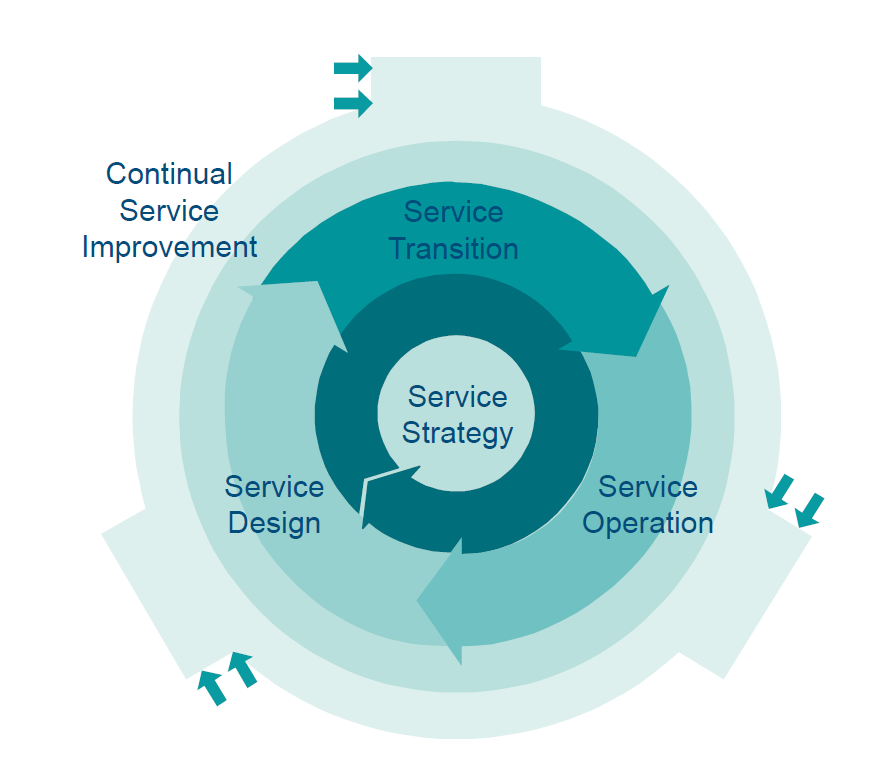
\includegraphics[width=\columnwidth]{Images/06169041-6a7c-4ae5-a525-146450101b65.PNG}\caption{Service Lebenszyklus}
~\protect\cite[S.~17]{Beims.2015}\label{fig:serviceLife}\end{figure} 
Abbildung \ref{fig:serviceLife} zeigt die Zusammenhänge bei der Gestaltung des IT-Service-Managements. Das Verhaltensmuster der Mitarbeiter in der IT-Organisation wird auf Basis des Service Lebenszyklus gebildet. Der Umgang mit den Ereignissen in der Serviceerbringung und demnach auch die Qualität der IT-Services wird durch diese Verhaltensmuster beeinflusst.  \\
Im Folgenden soll ein kurzer, inhaltlicher Überblick der einzelnen Elemente des Service Lebenszyklus gegeben werden.

\subsubsection{Elemente des Service Lebenszyklus}
\begin{itemize}
\item \textbf{Service Strategy~\cite[S.~17]{Beims.2015},~\cite[S.~14]{KarlMichaelGauch.24.03.2021}} 
\begin{itemize}
\item[•]Identifiziert Strategien, Prozesse und Kunden 
\item[•] Schöpft Chancen aus 
\item[•] Analyse der Vermögenswerte 
\item[•] Bildet den Ausgangspunkt für alle Aktivitäten des Service Lifecycle und bietet Unterstützung und Anleitung für Design, Entwicklung und Implementierung von Service Management
\end{itemize}
\end{itemize}
\begin{itemize}
\item \textbf{Service Design ~\cite[S.~18]{Beims.2015},~\cite[S.~14]{KarlMichaelGauch.24.03.2021}}
\begin{itemize}
\item[•]Setzt die Vorgaben aus Service Strategy um und liefert Vorgaben und Vorlagen für die Erstellung adäquater und innovativer IT-Services
\item[•]. Betrachtet sowohl die Gestaltung neuer und veränderter Services als auch der Service-Management-Prozesse 
\end{itemize}
\end{itemize}
\begin{itemize}
\item \textbf{Service Transition ~\cite[S.~18]{Beims.2015},~\cite[S.~14]{KarlMichaelGauch.24.03.2021}}
\begin{itemize}
\item[•]Stellt eine Anleitung und Prozessaktivitäten für den Übergang der Services in die Business-Umgebung bereit
\item[•] Behandelt auch Themen wie Veränderungen der Unternehmenskultur, Wissens- und
Risikomanagement
\end{itemize}
\end{itemize}
\begin{itemize}
\item \textbf{Service Operation ~\cite[S.~18]{Beims.2015},~\cite[S.~14]{KarlMichaelGauch.24.03.2021}}
\begin{itemize}
\item[•]Betrachtet das tägliche Geschäft des Servicebetriebs
\item[•]Behandelt die effektive und effiziente Lieferung bzw. Unterstützung von Services, mit dem Ziel, Mehrwert für Kunden und Service Provider zu erzielen
\item[•]Beinhaltet neben den klassischen Prozessen wie Incident oder Problem Management auch Themen wie Application Management und Technical Management sowie die Messung und Steuerung von Prozessen und Funktionen
\end{itemize}
\end{itemize}
\begin{itemize}
\item \textbf{Continual Service Improvement ~\cite[S.~18]{Beims.2015},~\cite[S.~14]{KarlMichaelGauch.24.03.2021}}
\begin{itemize}
\item[•]Dienstleistungen verbessern
\item[•]Kosteneffizienz verbessern
\item[•]Sich ändernde Geschäftsanforderungen erfüllen
\item[•]Qualitätsmanagement
\item[•] Verläuft über die gesamte Zeit des Service Lifcycles.
\end{itemize}
\end{itemize}
\begin{figure}[htb]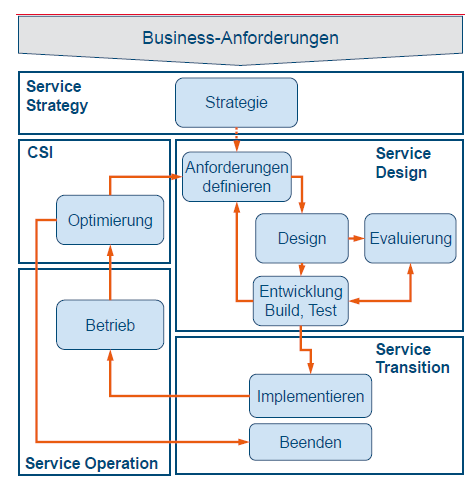
\includegraphics[width=\columnwidth]{Images/16724a53-da3e-455d-a7a2-ef43ced2e51e.PNG}\caption{Zusammenspiel der einzelnen Elemente im Service Lebenszyklus}
~\protect\cite[S.~18]{Beims.2015}\label{fig:zusammenspiel} \end{figure}
Abbildung \ref{fig:zusammenspiel} stellt das Zusammenspiel der einzelnen Elemente des Service Lebenszyklus dar und zeigt somit den Ablauf von ITIL. Zunächst müssen die Business Anforderungen benannt werden. Dadurch wird in dieser Phase bereits sichergestellt , dass jede Stufe des Service Lebenszyklus am Business orientiert ist. Es werden Strategien entwickelt, Chancen und Möglichkeiten identifiziert und Ziele definiert, um die Gestaltung neuer IT Services anzutreiben. 
Die Service Strategy umfasst fünf Prozesse: Service Portfolio Management, Strategy Management for IT Services, Demand Management und Business Relationship Management. Diese identifizieren durch unterschiedliche Prozessziele die Arten von Services, welche Kunden bzw. am Markt angeboten werden sollen. Zur Unterstützung werden dazu zwei Modelle hinzugezogen. Bei dem ersten hinzugezogenen Modell handelt es sich um das Kano Modell. Es beschreibt den Zusammenhang zwischen dem Erreichen bestimmter Eigenschaften eines Produktes / einer Dienstleistung und der erwarteten Zufriedenheit von Kunden \footnote{https://de.wikipedia.org/wiki/Kano-Modell-cite-note-1, Zugriff: 13.06.2021}. Das zweite Modell ist der 4P - Marketing Mix, welches sich mit der Produkt-, Preis-, Vertriebs- und Kommunikationspolitik beschäftigt. Das Ergebnis der Service Strategy sind Service Modelle, eine Business Impact Analyse sowie weitere Dokumente\footnote{ITIL On A Page, ITIL TrainingZone.com}. \\
Nachdem diese Stufe abgearbeitet ist, folgt das Service Design. Anhand der Ergebnisse aus der Service Strategy können nun konkrete Anforderungen definiert werden. In dieser Phase werden neue Services entworfen, aber auch Änderungen und/oder Verbesserungen vorhandener Services durchgeführt. 
Wie in Abbildung \ref{fig:zusammenspiel} dargestellt, handelt es sich in dieser Phase um einen iterativen Prozess. Die Anforderungen können dabei um weitere Punkte ergänzt werden. Diese Services müssen entwickelt und getestet werden, wodurch eine stetige Evaluierung stattfindet. Je nach Ergebnis der Evaluierung müssen die nun bestehenden Services gegebenenfalls nochmal verändert oder verbessert werden. Auch diese Disziplin besteht aus acht Prozessen, die die Entwicklung und Veränderung bzw. Verbesserung von Servicen durchführt: Design Coordination, Service Catalogue Management, Service Level Management, Availability Management, Capacity Management, IT Service Continuity Management, Information Security Management und Supplier Management. Die Ergebnisse dieser Phase sind unter anderem die sogenannten Service-Level Agreements, Architektur oder Service Design Packages\footnote{ITIL On A Page, ITIL TrainingZone.com}. 
\\
Die Service Transition verfolgt das Ziel, dass die entwickelten Services der letzten Phase aufgebaut und ausgerollt werden. Zudem wird durch geeignete Test- und Change Modelle sichergestellt, dass Änderungen an den Services koordiniert ablaufen. Die Ergebnisse dieser Phase sind unter anderem ein Content-Management-System, ein Service Knowledge System oder ein Change schedule.\\
Nachdem die Services entwickelt und verschiedene Systeme für einen reibungslosen Ablauf  bereitgestellt sind, dient die Service Operation Stufe dazu, dass die IT Services effektiv und effizient erbracht werden. In dieser Stufe müssen Anwenderfragen erfüllt und Probleme gelöst werden. Auch hier stehen fünf Prozesse zur Verfügung, die durch unterschiedliche Funktionen gemeinsam das Ziel erarbeiten: Incident Management, Problem Management, Access Management, Request Fulfilment und Event Management. In dieser Phase entstehen vor allem technische Dokumentationen und Übungsmaterial\footnote{ITIL On A Page, ITIL TrainingZone.com}. 
\\
Infolge der vorherigen Stufen können immer wieder Qualitätsmängel auftreten. Um diesen entgegen zu wirken und aus den Erfolgen sowie Misserfolgen der Vergangenheit zu lernen, wird im Continual Service Improvement gezieltes Qualitätsmanagements betrieben\footnote{ITIL On A Page, ITIL TrainingZone.com}. 
\subsubsection{Rollen im Service Lifecycle} 
Aufgrund der hohen Anzahl an Phasen und Prozesse im Service Lifecycle, benötigt es die Definition von unterschiedlichen Rollen, die in den fünf Phasen verschiedene Aufgaben übernehmen. Der ITIL One Pager benennt vier generische Rollen innerhalb des Service Lifecycles: 
\begin{itemize}
\item[•]\textbf{Service Owner}\\
Verantwortlich gegenüber dem Kunden für die Initiierung, den Übergang und die laufende Wartung sowie Unterstützung eines  Dienstes und Support eines bestimmten Services ~\cite[S.~9]{KarlMichaelGauch.24.03.2021}.
\item[•]\textbf{Process Owner} \\
Verantwortlich, dass Service seine Ziele enstprechend der Prozessdefinition erfüllt ~\cite[S.~9]{KarlMichaelGauch.24.03.2021}.
\item[•]\textbf{Process Manager}\\
Verantwortet das Operativemanagement eines Prozesses. Es kann mehrere Process Manager für einen Prozess geben ~\cite[S.~9]{KarlMichaelGauch.24.03.2021}. 
\item[•]\textbf{Process Practitioner}\\
Die Durchführung einer oder mehrerer Prozessaktivitäten liegt in dessen Verantwortung ~\cite[S.~9]{KarlMichaelGauch.24.03.2021}.
\end{itemize}
\subsubsection{Key Performance Indicators} 
Ein Key Performance Indicator (KPI) ist eine Leistungskennzahl, durch die eine Analyse zu Erfolg und Misserfolg eines Unternehmens durchgeführt werden kann. Im Bereich ITIL v3 werden in jeder Stufe des Service Lebenszyklus KPIs ermittelt, um festzustellen wie gut oder schlecht die Services in der jeweiligen Phase sind. 
In den folgenden Tabellen werden für jede Phase beispielhaft KPIs dargestellt. 
\begin{table}[!ht]
  \caption{Beispielhafte KPIs der Service Strategy}
  \label{tab:freq_1}
  \begin{tabular}{c|c}
    \toprule
    \textbf{Leistungskennzahlen}&\textbf{Definition}\\
    \toprule
    \shortstack{Anzahl geplanter\\ neuer Services }& \shortstack{Anzahl neu entwickelter \\Services, die aufgrund\\ eines strategischen Reviews \\initiiert worden sind} \\
    \hline
   \shortstack{ Anzahl von \\Neukunden} &\shortstack{Anzahl neu\\ gewonnener Kunden} \\
    \hline
    \shortstack{Anzahl von\\ Kundenbeschwerden }& \shortstack{Anzahl der \\eingegangenen \\Kundenbeschwerden}\\
    \hline
    \shortstack{Einhaltung \\Projektressourcen } &\shortstack{Anteil der Kosten,\\ der die geplanten\\ Projektkosten überschreitet}\\
  \toprule
\end{tabular}
\end{table}
Tabelle \ref{tab:freq_1} zeigt Beispiele, die die Leistung eines Unternehmens in der Service Strategy bewertbar macht. 

\subsection{Qualitätsicherung in ITIL - Lara}
Qualitätssicherung spielt im ITIL Framework eine zentrale Rolle.
Dies ist darauf zurückzuführen, dass ein Grundgedanke von ITSM
darin besteht die Qualität und Quantität von IT-Services zu planen,
überwachen und steuern \cite{Beims.2015}. An dieser Stelle wird beschrieben in
welchen Bereichen von ITIL Qualitätssicherung verortet ist, welche Tätigkeiten sie umfasst und nach welchen Ansätzen diese strukturiert und ausgeführt werden können.

\subsubsection{Qualitätssicherung im ITIL-Prozess}
Wie bereits in Kapitel \ref{sec:intro} beschrieben, ist ITIL Service Management in sechs Bereiche aufgeteilt, Service
Strategy, Service Design, Service Transition, Service Operation, welche
zeitlich nacheinander ablaufen, und Continual Service Improvement
(CSI), welcher parallel zu den anderen Bereichen kontinuierlich
bespielt wird. Qualitätssicherung ist dabei hauptsächlich
im Bereich CSI verortet, steht jedoch auch in engem Zusammenhang mit den vier anderen Bereichen. Qualitätssicherung ist in \textit{Service Strategy} , \textit{Service Design},
\textit{Service Transition}, \textit{Service Operation} integriert, da alle in deren Rahmen durchgeführten Aktivitäten so ausgerichtet sein sollen, dass die eine hohe Produktqualität gewährleistet wird \cite{Beims.2015}. Die Sicherstellung einer hohen Servicequalität wird dabei zunächst in der Planung berücksichtigt, indem die Wünsche der Zielgruppe betrachtet werden. Anschließend werden die geplanten Qualitätsziele konkret umgesetzt. Zudem spielt die Qualitätssicherung im gesamten ITIL-Prozess eine Rolle, da die Aktivitäten fünf Einzelbereiche als Grundlage für das CSI dienen und Ergebnisse des CSI wiederum den Anstoß für weitere Aktivitäten in den Bereichen liefert \cite{Beims.2015}. Das genaue Zusammenspiel der Einzelbereiche und des CSI wird im nächsten Kapitel im Rahmen der Erklärungen zum CSI Prozess genauer erläutert. Vereinfacht kann gesagt werden, dass Qualitätssicherung in alle Aktivitäten des Service Managements integriert ist.

\subsubsection{Continuous Service Improvement}
Das CSI ist ein Kreislauf bestehend aus den grundlegenden vier Aktivitäten \textit{Plan}, \textit{Do}, \textit{Check}, \textit{Act} \cite{Beims.2015}. Der Prozess beginnt mit der Phase \textit{"Plan"}, welche das Festlegen von Zielen, Aktivitäten und Verantwortlichkeiten umfasst, dann folgt in \textit{"Do"} die Umsetzung der Pläne und die Dokumentation der Umsetzung. Anschließend wird mit dem \textit{"Check"} überprüft, wie die Pläne umgesetzt wurden und die Ergebnisse dieser Messung werden dokumentiert. In \textit{"Act"} werden die ermittelten Ergebnisse betrachtet und Maßnahmen zur Korrektur möglicher Abweichungen definiert. Dies bildet wiederum die Grundlage für erneute Planungen, wodurch der Kreislauf von vorne beginnt. Auf diese Art und Weise kann ein Service nach und nach immer wieder verbessert und auch über einen längeren Zeitraum an sich verändernde Anforderungen der Nutzer angepasst werden. So wird mithilfe des beschriebenen Kreislaufes die Qualität des Produktes gesichert. \cite{Beims.2015}\\

Um die Aktivitäten im CSI noch genauer zu beschreiben, existiert das siebenstufige Modell des CSI-Improvement Prozesses \cite{Beims.2015}. Dieses ist in Abbildung \ref{fig:CSIprozess} dargestellt. 
\begin{figure}[htb]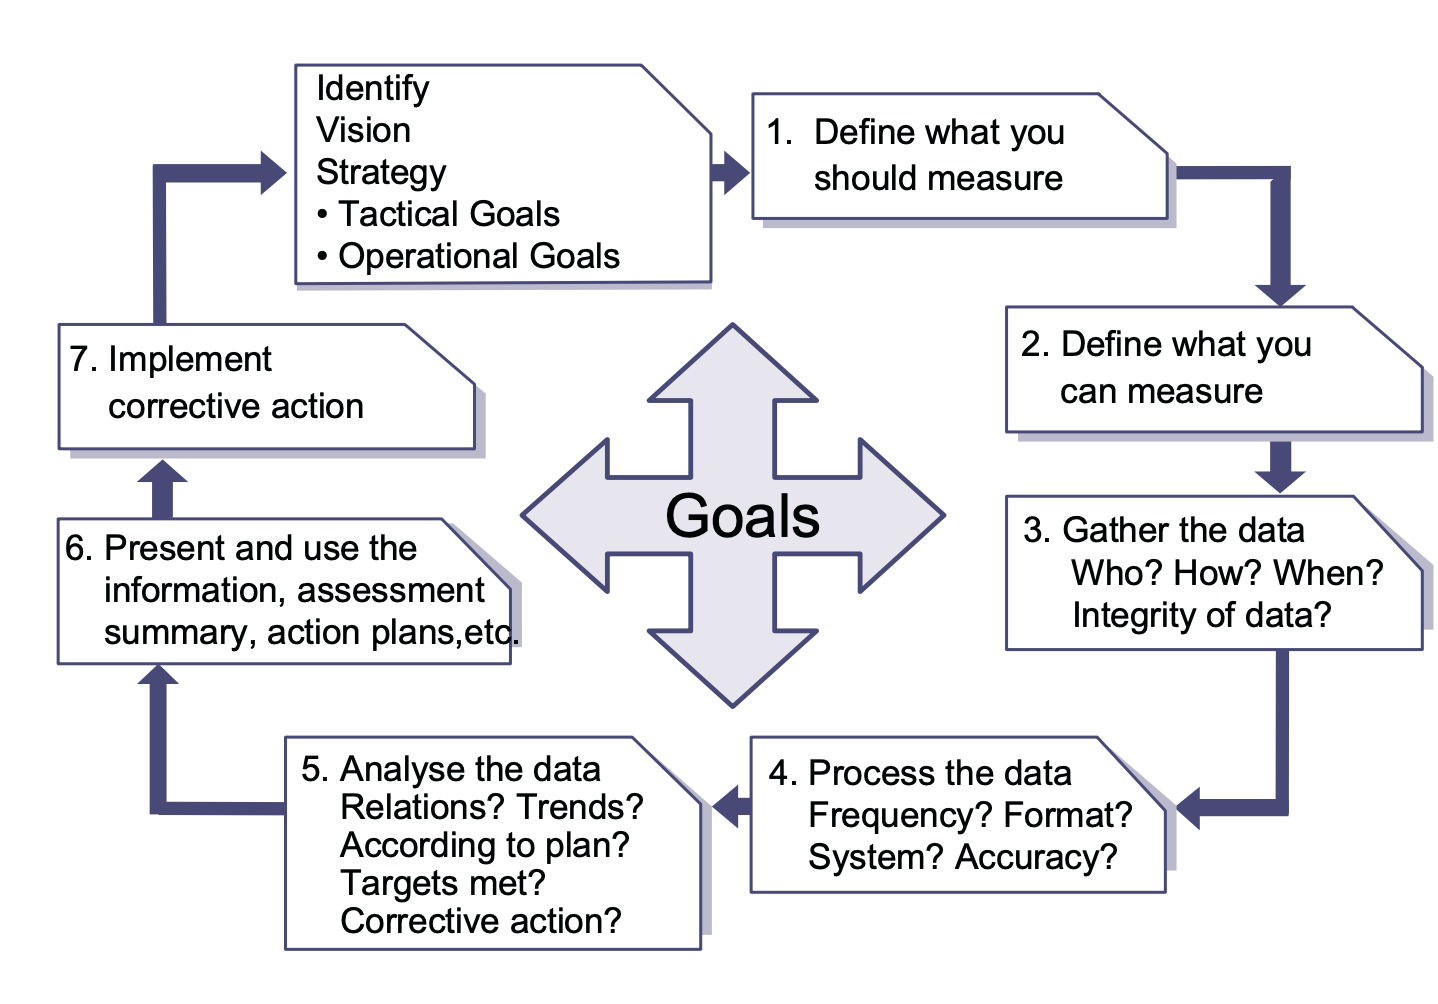
\includegraphics[width=\columnwidth]{CSI_Prozess.png}\caption{CSI-Improvement Prozess}
~\protect\cite[S.45]{Beims.2015}\label{fig:CSIprozess}\end{figure} 
Dort ist zu sehen, dass alle sieben Stufen auf die grundlegenden Ziele bezogen sind, auf denen der CSI-Improvement Prozess aufgebaut ist. Die Ziele bestehen darin, dass anhand der "strategischen, taktischen und operationellen Ziele des Unternehmens" ~\cite[S.~44]{Beims.2015} definiert werden, welche Daten zur Qualitätssicherung erhoben werden sollen. Zudem sollen hierzu passende Messmethoden und Kriterien festgelegt werden, sodass Messergebnisse als Entscheidungsgrundlage genutzt werden können, um die Qualität des Services sicherstellen zu können \cite{Beims.2015}.

Im linken oberen Teil der Grafik ist zu sehen, dass im Kreislauf ein Prozessschritt integriert ist, welcher keine der sieben Stufen des CSI-Prozesses ist, jedoch zwingend notwendig für den CSI-Prozess ist. Dies ist der Schritt, in welchem die anderen Bereiche mit dem CSI zusammenspielen, indem zunächst in jedem Bereich die jeweiligen Ziele, die Vision und die Strategie festgelegt werden aufgrund derer die Umsetzung des Produktes stattfindet. Diese muss als erstes durchlaufen werden, um mit dem Kreislauf und den eigentlichen CSI Aktivitäten starten zu können. Anhand der Konzepte, die in den einzelnen Bereichen festgesetzt wurden, erfolgt anschließend der erste CSI Schritt, die Festlegung von Kennzahlen, die gemessen werden sollen \cite{Beims.2015}. Dies resultiert in einer Liste, in der Metriken aufgelistet sind, die zur Überwachung der Zielerreichung erfasst werden sollen. Anschließend wird in Schritt zwei analysiert welche dieser Metriken tatsächlich gemessen werden können. Dies ist abhängig vom dafür notwendigen Zeitaufwand und der dafür benötigten Technik. Dabei muss abgewogen werden, welche Kennzahlen gemessen werden können und bei welcher Messung mehr Ressourcen benötigt werden als der Nutzen der Messung wert ist. Eine Ablehnung der Messung aufgrund eines schlechten Kosten-Nutzen-Verhältnisses könnte beispielsweise erfolgen, wenn für eine Messung eine kostenintensive Spezialsoftware benötigt wird. Überwiegen die Kosten dieser Spezialsoftware die Gewinne, die durch die Optimierung des gemessenen KPIs erzielt werden können, sollte auf die Messung verzichtet werden. Anschließend werden die festgelegten Metriken gemessen und somit erfasst wie effektiv und effizient der Service ist und Prozesse ablaufen \cite{Beims.2015}. Hierbei ist eine enge Zusammenarbeit zwischen Service Operation und CSI erforderlich, wobei zu Beginn festgelegt wird wann und wie die Daten erfasst werden und wer für die Datenerfassung zuständig ist. Für die Datenerfassung kann außerdem Software-Testing eingesetzt werden, wodurch ebenfalls eine direkte Schnittstelle zur Entwicklung und möglicherweise ein Software-Testing Team entsteht. Nach der eigentlichen Messung werden aus gemessenen Daten Informationen abgeleitet, welche später zur Bewertung der Messung herangezogen werden können. Hierzu werden die erfassten Daten gruppiert und aufgearbeitet. Daraufhin können die Daten analysiert werden, indem die Messungen mit den zuvor definierten Zielen verglichen werden. Dabei wird ermittelt ob die Ziele erreicht wurden, ob sich der Service zum Positiven oder zum Negativen entwickelt hat und ob Korrekturen vorgenommen werden sollten. Wurden alle Erwartungen und Ziele erfüllt kann der CSI Prozess an dieser Stelle vorzeitig wieder beim Schritt des Messens beginnen. Sind Korrekturmaßnahmen notwendig müssen zunächst alle betroffenen Mitarbeiter über die Ergebnisse aufgeklärt werden. Anschließend werden gemeinsam Möglichkeiten diskutiert, wie Korrekturen vorgenommen werden können und es werden Maßnahmen festgelegt und von allen Beteiligten genehmigt. Ist dieser Schritt abgeschlossen folgt die Umsetzung der festgesetzten Korrekturmaßnahmen und nach Abschluss dieser Tätigkeiten startet der CSI Prozess von Neuem.\cite{Beims.2015}\\

Im gesamten Prozess ist es dabei von großer Wichtigkeit, dass ein Verantwortlicher für den Qualitätssicherungs-Prozess festgelegt wird, welcher als Ansprechpartner für andere Teams fungiert. Dieser Verantwortliche ist dabei auch verantwortlich für die weitere Rollenzuweisung, dem Management des Monitoring, der Sicherstellung der CSI-Aktivitäten und der Maßnahmenpriorisierung. Zudem erstellt und pflegt er den sogenannten Service Improvement Plan, in dem aufbauend auf regelmäßigen Terminen der Stakeholder vorgesehene Verbesserungsmaßnahmen dokumentiert werden. \cite{Beims.2015}

\subsubsection{Testing - René }
\label{sec:testing_background}
Der Testing Prozess stellt die Einhaltung des Vertrags, welcher
mit dem Kunden über die Qualitätsanforderungen abgeschlossen
wird, sicher. Der Nutzen des Kunden steht daher im Mittelpunkt. Es
kann dabei zwischen zwei verschiedenen Kategorien unterschieden
werden: Die \textit{Utility} (Nützlichkeit) und die \textit{Warranty} (Garantie) \cite{Beims.2015}. Die Utility befasst sich dabei direkt mit den vom Kunden erwarteten
Services, während die Warranty die Verfügbarkeit dieser
Services ins Auge fasst. Aus diesen beiden Kategorien leitet sich die
Notwendigkeit ab, zum einen das Produkt selbst zu testen und zum anderen
die Strukturen, welche die Nutzung des Produkts ermöglichen. Dazu
gehören unter anderem interne Services, sowie das Deployment-Umfeld. Die Tests zielen dabei darauf ab, Fehler zu identifizieren und zu evaluieren ob vom Kunden gestellte Anforderungen wie gewünscht
erfüllt wurden. Final müssen die erhobenen Ergebnisse an
die verantwortliche Personen gemeldet werden, um Fehlerquellen
möglichst schnell zu beheben. Da in vielen Bereichen getestet werden
muss, um diese Kriterien sicherzustellen, ist eine umfassende
Teststrategie unabdingbar. 

Um eine geeignete Teststrategie zu entwickeln, empfiehlt es sich etablierte Testmodelle wie zum Beispiel das Wasserfallmodell oder agile Testansätze zu nutzen. Bei der Entwicklung einer geeigneten Teststrategie wurde sich im Zuge dieser Arbeit an das Service V-Modell gehalten, welches in Abbildung \ref{fig:vmodell} dargestellt ist und vom Standardwerk zu ITIL\cite{Beims.2015} als Best-Practice-Modell vorgestellt wird. Dieses definiert zu jedem Design- bzw. Entwicklungsschritt der einzelnen Services eine passenden Test. Dabei kann dieser Prozess in fünf Abschnitte unterteilt werden: \\

Der \textit{Component Test} wird parallel zur eigentlichen Service Entwicklung definiert. Dieser prüft, ob die einzelnen Komponenten, bzw. eine Gruppe an Komponenten, die geforderte Spezifikationen erfüllt. Es wird die direkte technische Umsetzung der Services getestet. Im \textit{Release Package Test} wird anschließend getestet, ob die erstellten Services fehlerfrei bereitgestellt (deployed) werden können. Der \textit{Operational Readiness Test} bezieht sich auf die Ressourcen, welche vorhanden sein müssen, um den Service bereitzustellen. Damit sind nicht nur technische, sondern auch Humanressourcen gemeint. Es wird also genauso danach gefragt, ob genügend Speicher vorhanden ist, wie auch, ob der Support für den jeweiligen Service geleistet werden kann. Der \textit{Acceptance Test} erfolgt im direkten Zusammenspiel mit dem Kunden. Hier wird sichergegangen, dass der Service alle gestellten Kundenanforderungen zufriedenstellend erfüllt. An letzter Stelle steht die \textit{Service Validierung}. Dabei wird geprüft, ob der Service alle mit dem Kunden vereinbarten Verträge erfüllt. 

\begin{figure}[th]
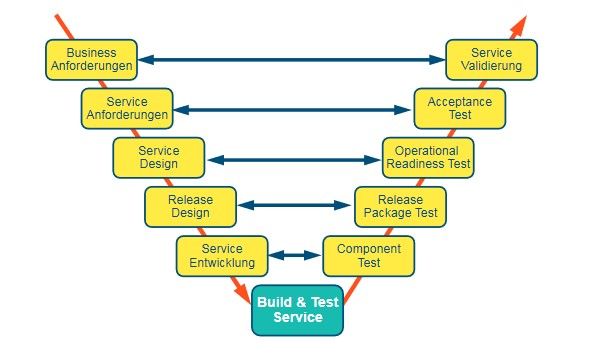
\includegraphics[width=\columnwidth]{images/V-Modell.jpg}
\caption{Service V-Modell \cite{Beims.2015} }
\label{fig:vmodell}
\end{figure}

\section{Praktische Durchführung}
\label{chapter_praktischedurchführung}
In Kapitel 2 wurden zunächst die theoretischen Grundlagen von ITIL und Qualitätssicherung und Testing in ITIL erläutert. Diese fanden im Rahmen des Projektes im Planspiel TopBlogAG praktische Anwendung. Bei dem genannten Planspiel wurden die Prozesse in einer IT-Firma aufbauend auf dem ITIL Framework mit fünf verschiedenen Teams simuliert. Die Teams waren das \textit{Business-Team}, das \textit{Entwicklungs-Team}, das \textit{Service-Desk Team}, das \textit{IT Operations Team} und das \textit{Qualitätssicherungs-Team}. In diesem Abschnitt wird beschrieben wie die theoretischen Konzepte der Qualitätssicherung und Testing in ITIL vom Qualitätssicherungsteam praktisch im Planspiel umgesetzt wurden.


\subsection{CSI im Planspiel - Lara}
Um die Aufgabe der Qualitätssicherung zu erfüllen, wurde vom Qualitätssicherungsteam im Planspiel der CSI-Improvement-Prozess als Grundlage genutzt, welcher zusätzlich um Testing-Aktivitäten ergänzt wurde. In diesem Abschnitt wird beschrieben wie CSI im Projekt angewandt wurde.

In Kapitel 2.2.2 ist der siebenstufige CSI-Improvement Prozess beschrieben. Dieser bildete im Projekt die Grundlage für die Durchführung der Qualitätssicherung. Zunächst wurden vom Business Team im Bereich der Service Strategy und des Service Designs und dem Entwicklungsteam in der Umsetzungsplanung und der Service Transition-Planung der Grundstein für den eigentlichen CSI-Prozess gelegt. Dabei fand eine enge Kommunikation zwischen den Teams und der Qualitätssicherung statt, um sicherzugehen, dass alle Ziele korrekt verstanden wurden. 

Diese Grundlage wurde dazu genutzt anschließend KPIs zu definieren, welche während der Entwicklung und der Laufzeit des Systems gemessen werden sollten, um die Service Qualität sicherstellen zu können. Hierzu wurden zunächst das Service Portfolio und die darin definierten SLAs mit dem Business Team diskutiert und in messbaren KPIs festgehalten. Anschließend wurde der Service Katalog und die Service Transition Strategie mit dem Entwicklungsteam besprochen und daraus weitere KPIs definiert. Zudem wurden Gespräche mit dem IT Operations Team und dem Service Desk geführt, um die festgelegten KPIs zu verbessern und durch weitere Anforderungen zu ergänzen. Nachdem die KPIs definiert wurden fand ein Austausch mit den Verantwortlichen im IT Operations Team und im Entwicklungsteam statt, in dem geklärt wurde, welche Metriken gemessen werden können. In Tabelle \ref{tab:ortitot} und \ref{tab:ortsd} sind Auszüge der entstandenen KPI-Dokumentation zu finden. Nachdem nun definiert war, welche KPIs gemessen werden sollen wurde definiert, welche Tests und welches Monitoring dafür notwendig ist. Dabei wurde der im nächsten Abschnitt beschriebene Testing Prozess geplant. Die dort beschriebenen Tests wurde neben dem Monitoring des IT Operations Team durchgeführt um KPIs zu messen. Die so festgelegten KPIs, Verantwortlichkeiten und Prozesse wurden abschließend für die Schritte eins bis drei des CSI-Improvement Prozesses in einem Dokument zusammengefasst. Dieses zeigt die Metriken, deren Messverfahren und die für die Messung verantwortlichen Bereiche und ist im Anhang zu finden. Dabei ist zu sehen, dass in einer zusätzlichen Spalte vom Qualitätssicherungsteam vor der tatsächlichen Messung bereits eine Qualitätseinstufung vorgenommen wurde. Diese wurde anhand der Informationen der Planungen der anderen Teams erstellt und dient im Verlauf des Prozesses dazu einstufen zu können, welcher Messwert was für die tatsächliche Qualität des Services bedeutet. Dieses erstellte Übersichtsdokument bildet die Service Quality Policy für das Projekt. Mithilfe derer kann in der Analysephase anhand von konkreten Werte darüber entschieden werden, ob Verbesserungsmaßnahmen durchgeführt werden müssen. 

Anschließend erfolgte die tatsächliche Messung der Daten durch das IT Operations Team, das Service Desk Team und das Testing im Qualitätssicherungsteam. Die erfassten Daten werden anschließend von den jeweiligen Verantwortlichen aufgearbeitet, da die einzelnen Bereiche den besten Überblick über die Daten haben und diese am besten in einen Kontext setzen können. Um eine einheitliche Dokumentation der verarbeiteten Daten für die spätere Analyse zu gewährleisten, wurde ein für alle zugängliches Dokument erstellt, in welchem bei jeder Messung der gemessene KPI, die erfassten Werte, der Zeitpunkt der Messung und der Dokumentierende eingetragen werden. Zusätzlich wird in diesem Dokument direkt eine Einstufung der KPI-Qualität anhand der KPI-Übersichtstabelle vorgenommen. 

Für die anschließende Analysephase wurde ein Ablaufplan erstellt, welcher allen Messverantwortlichen zugänglich ist und beschreibt, wie mit verschiedenen Messwerten umgegangen wird. Dieser Plan ist in Anhang (?) zu finden und beschreibt, dass bei einer Einstufung des Messwertes als hohe Qualität keine weiteren Analysen und Maßnahmen erforderlich sind. Auf diese Weise kann auch im praktischen Projekt der CSI-Prozess bei guter Qualität direkt beim Schritt eins wieder begonnen werden, wie es der theoretische ITIL CSI Ablauf vorsieht. Wird die Qualität jedoch als mittel oder niedrig eingestuft wird beschrieben, wie in der Analyse-Phase vorgegangen wird. Dabei wird bei Werten von mittlerer Qualität zunächst betrachtet ob aktuell Werte mit niedriger Qualität bestehen. Ist dies der Fall werden die KPIs von mittlerer Qualität depriorisiert, jedoch dennoch die Verantwortlichen für die jeweilige Funktion über die Qualitätsmessung informiert, um ein Bewusstsein zu schaffen. Bestehen keine anderen Werte von niedriger Qualität oder wurde ein niedriger Wert gemessen startet der konkrete Analyseprozess. Hierzu wird zunächst der Verantwortliche der Funktion hinter der gemessenen KPI informiert und mit in die Messungstabelle eingetragen. Anschließend informiert dieser Verantwortliche alle Stakeholder und bespricht zusammen mit diesen, welche Maßnahmen für die Verbesserung der Metrik durchgeführt werden sollen. Diese Planung wird im, vom Qualitätssicherungsteam bereitgestellten, Service Improvement Plan festgehalten. Dabei wird zunächst die Planungsänderung beschrieben und alle an der Planung Beteiligten werden in der dafür vorgesehenen Spalte eingetragen. Nach der Planung informieren die Planenden die anderen an der Maßnahme beteiligten Teams. Diese müssen der Maßnahme zustimmen, oder die Maßnahme ablehnen, was wiederum im Service Improvement Plan festgehalten wird. Wurde die Planung abgelehnt muss dies begründet werden, um wiederum eine neue Verbesserungsplanung zu starten. Bei Zustimmung wird der Beschluss der Maßnahme kommuniziert, um in Strategie-, KPI- und Releaseplanungen aufgenommen werden zu können. Ist dieser Schritt abgeschlossen beginnt der CSI-Prozess von neuem.

\subsection{Testing-Rene}

In diesem Abschnitt wird aufgeführt, wie mithilfe des Service V-Modells Tests entwickelt und durchgeführt wurden. 

\subsubsection{Component Test}
Die Component Tests beziehen sich wie in Abschnitt \ref{sec:testing_background} beschrieben auf die direkte Implementierung der Service-Anforderungen. Die Frage, welche die Component Tests beantworten sollen lautet daher: Werden die Anforderungen in der Implementierung zufriedenstellend umgesetzt? Um diese Frage zu beantworten wurde zunächst für jede Anforderung an den Service eine Schwachstellenanalyse durchgeführt. Diese Schwachstellen wurden anschließend mit einem Risikostatus gewichtet. Dabei wurden vier verschiedene Gewichtungen definiert, welche hier aufsteigend aufgelistet sind: \textit{Geringfügig, Mittelmäßig, Kritisch} und \textit{Katastrophal}. Diese Gewichtung wurde vorgenommen, um die Dringlichkeit einer Anpassung zu dokumentieren. Zu jeder Anforderung wurde weiterhin ein oder mehrere Annahmekriterien definiert, welches sich direkt aus dem vom Business Team erstellten Service Portfolio ableiten. Im folgenden wurden die Component Tests durch den/die Softwaretester*in durchgeführt und dokumentiert, ob der Test bestanden wurde und von wem er durchgeführt wurde. Weiterhin wurden Auffälligkeiten genau dokumentiert, um eventuelle Fragen zu klären oder mehr Informationen zu gescheiterten Tests zu liefern. Die Testergebnisse wurden gebündelt für einzelene Komponenten an den \textit{Head of Development} zurückgemeldet. Weiterhin wurde eine Metrik für die Qualität einzelner Komponenten eingeführt. Nach dieser hat eine Komponente eine Qualität von 100\% , wenn alle auf ihr ausgeführten Tests bestanden sind. Bei der Berechnung der Metrik wird die Gewichtung des Risikos mit einbezogen indem den einzelnen Gewichtungen aufsteigend Werte von eins bis vier zugewiesen wurden. Wurde ein Test nicht bestanden, wird der gewichtete Anteil von den 100\% abgezogen. Als zufriedenstellende Qualität einer Komponente wurde ein Wert von über 95\% festgelegt. Eine mittlere Qualität besteht bei 85-95\% und eine niedrige Qualität bei unter 85\%.  Ein beispielhafter Auszug der Dokumentation eines Component Tests findet sich in Tabelle \ref{table:component}. 

\begin{table*}[]
\begin{tabular}{|l|l|l|l|l|l|l|}
\hline
\textbf{Komponente} & \textbf{Annahmekriterium}                                                                                            & \textbf{Schwachstellenanalyse}                                                                                                & \textbf{Risikobewertung} & \textbf{Testergebnis} & \textbf{Verantwortlich}                                                      & \textbf{Notiz} \\ \hline
Registrierung      & \begin{tabular}[c]{@{}l@{}}Reg. über: \\ E-Mail\\ Passwort\\ Name\\ Nachname\\ Benutzername\end{tabular}              & \begin{tabular}[c]{@{}l@{}}Es können Texte welche \\ keine E-Mail Adresse sind\\ als E-Mail angegeben \\ werden.\end{tabular} & Katastrophal             & Bestanden             & \begin{tabular}[c]{@{}l@{}}Software-Testerin\\ Lara Krautmacher\end{tabular} & -                    \\ \hline
Registrierung      & \begin{tabular}[c]{@{}l@{}}Person bekommt \\ nach Registrierung\\ einen Bestätigungs-\\ link\\ per Mail\end{tabular} & \begin{tabular}[c]{@{}l@{}}Link in E-Mail ist nicht\\ gültig oder E-Mail \\ kommt nicht an.\end{tabular}                      & Kritisch                 & Bestanden             & \begin{tabular}[c]{@{}l@{}}Software-Testerin\\ Elena Kirsch\end{tabular}     & -                    \\ \hline
...                & ..                                                                                                                   & ...                                                                                                                           & ...                      & ...                   & ...                                                                          & ...                  \\ \hline
\end{tabular}
\caption{Component Tests Registrierung}
\label{table:component}
\end{table*}  


\begin{comment}
\begin{itemize}
\color{red}
\item Weiterhin wurde der interne Service des Service Desks, das Redmine Portal, getestet. Hier wurde ähnlich vorgegangen
\end{itemize}

\end{comment}



\subsubsection{Release Package Test}

Für die Durchführung der Release Package Tests ist in erster Linie die \textit{Release- und Deployment Managerin} verantwortlich. Dazu wurden jedoch von der Qualitätssicherung KPIs definiert, welche eine Aussage über den Release Prozess treffen.  Der erste KPI betrifft die Anzahl erfolgreicher Deployments. Diese Metrik wird in Prozent erfasst und nutzt folgende Staffelung: Eine hohe Qualität ist erreicht, wenn der KPI größer als 95\% ist. Eine mittlere Qualität besteht bei genau 95\% und eine niedrige Qualität bei unter 95\%. Der zweite KPI ist die Dauer der Deployments in Minuten. Hier besteht eine hohe Qualität bei weniger als 1 Minute 20 Sekunden, eine mittlere bei genau 1 Minute 20 Sekunden und eine niedrige Qualität bei mehr als 1 Minuten 20 Sekunden Deployment-Zeit. Diese Zeit wurde in Absprache mit dem IT Operations Team getroffen. 

\subsubsection{Operational Readiness Test}

Da sich der \textit{Operational Readiness Test} auf Humanressourcen sowie technische Ressourcen bezieht, richtet er sich an das Service Desk und IT Operations Team. Zum einen wird getestet, ob das Service Desk in der Lage ist eingehende Anfragen zufriedenstellend zu bearbeiten. Zum anderen wird geprüft, ob die technischen Komponenten, welche einzelne Services zur Verfügung stellen, den gestellten Anforderungen gerecht werden. Das Qualitätssicherungsteam hat hierzu ähnlich wie bei den Release Package Tests KPIs definiert, welche von den beiden anderen Teams beobachtet werden können. Diese finden sich in den Tabellen \ref{tab:ortitot} und \ref{tab:ortsd}. Die KPIs wurden ebenfalls aus dem Service Portfolio abgeleitet, um die im selbigen gestellten Anforderungen zu erfüllen. 

\begin{table*}[]
\begin{tabular}{|l|l|l|}
\hline
\textbf{KPI} &
  \textbf{Metrik} &
  \textbf{Qualitätseinstufung} \\ \hline
Serviceverfügbarkeit &
  \begin{tabular}[c]{@{}l@{}}Verfügbarbeit in Stunden / \\ Anzahl der Stunden pro Monat \\ in Prozent\end{tabular} &
  \begin{tabular}[c]{@{}l@{}}Niedrige Qualität: \textless{}98\\ Mittlere Qualität: \textgreater{}=98\\ Hohe Qualität: \textgreater{}99\end{tabular} \\ \hline
Mean Time To Failure (MTTF) &
  \begin{tabular}[c]{@{}l@{}}Summe( Uptimeende - Uptimestart) / \\ Anzahl der Fehler seit Start des Services\\ in Tagen\end{tabular} &
  \begin{tabular}[c]{@{}l@{}}Niedrige Qualität: \textless{}10\\ Mittlere Qualität: =10\\ Hohe Qualität: \textgreater{}10\end{tabular} \\ \hline
Mean Time To Recover (MTTR) &
  \begin{tabular}[c]{@{}l@{}}Summe(Fehlerende - Reperaturstart)/ \\ Anzahl der Fehler seit Start des Services\\ in Stunden\end{tabular} &
  \begin{tabular}[c]{@{}l@{}}Niedrige Qualität: \textgreater 1\\ Mittlere Qualität: = 1 \\ Hohe Qualität: \textless{}1\end{tabular} \\ \hline
Mean Time Between Failures (MTBF) &
  \begin{tabular}[c]{@{}l@{}}Summe(Fehlerstart - Uptimestart)/\\ Anzahl der Fehler seit Start des Services\\ in Tagen\end{tabular} &
  \begin{tabular}[c]{@{}l@{}}Niedrige Qualität: \textless 7\\ Mittlere Qualität: = 7\\ Hohe Qualität: \textgreater 7\end{tabular} \\ \hline
Antwortzeit bei Aufruf der Seite &
  \begin{tabular}[c]{@{}l@{}}Http response - http request / \\ Anzahl http requests\\ in Sekunden\end{tabular} &
  \begin{tabular}[c]{@{}l@{}}Niedrige Qualität: =1\\ Mittlere Qualität: \textgreater{}0,1 \\ Hohe Qualität: \textless{}=0,1\end{tabular} \\ \hline
\end{tabular}
\caption{OR Test KPIs für IT Operations}
\label{tab:ortitot}
\end{table*}

\begin{table*}[]
\begin{tabular}{|l|l|l|}
\hline
\textbf{KPI} &
  \textbf{Metrik} &
  \textbf{Qualitätseinstufung} \\ \hline
\begin{tabular}[c]{@{}l@{}}Durchschnittliche Kosten pro \\ Bearbeitung einer Kundenanfrage\end{tabular} &
  \begin{tabular}[c]{@{}l@{}}Lohn für Bearbeiter/\\ Anzahl Anfragen\\ in Euro\end{tabular} &
  \begin{tabular}[c]{@{}l@{}}Niedrige Qualität: \textgreater{}=10\\ Mittlere Qualität: \textgreater{}=5\\ Hohe Qualität: \textless 5\end{tabular} \\ \hline
\begin{tabular}[c]{@{}l@{}}Anzahl der bearbeiteten \\ Kundenanfragen pro Monat\end{tabular} &
  \begin{tabular}[c]{@{}l@{}}Anzahl der bearbeiteten\\ Kundenanfragen pro Monat\end{tabular} &
  \begin{tabular}[c]{@{}l@{}}Niedrige Qualität: \textless{}=50\\ Mittlere Qualität: \textless{}=100\\ Hohe Qualität: \textgreater 100\end{tabular} \\ \hline
\begin{tabular}[c]{@{}l@{}}Anteil der direkt gelösten\\ Kundenanfragen, die nicht\\ an einen Experten\\ weitergeleitet wurden\end{tabular} &
  \begin{tabular}[c]{@{}l@{}}100 - Weitergeleitete Anfragen/\\ Kundenanfragen pro Monat\\ in Prozent\end{tabular} &
  \begin{tabular}[c]{@{}l@{}}Niedrige Qualität: \textless{}80\\ Mittlere Qualität: \textless{}=90\\ Hohe Qualität: \textgreater{}90\end{tabular} \\ \hline
\begin{tabular}[c]{@{}l@{}}Durschnittliche Dauer\\ bis eingereichter Artikel\\ geprüft wird\end{tabular} &
  \begin{tabular}[c]{@{}l@{}}SummeAllerArtikel(Prüfung\\ des Artikels -\\ Einreichen des Artikels)/\\ Anzahl aller Artikel\\ in Stunden\end{tabular} &
  \begin{tabular}[c]{@{}l@{}}Niedrige Qualität:\textgreater{}=12\\ Mittlere Qualität: \textless{}12\\ Hohe Qualität: \textless{}=1\end{tabular} \\ \hline
\begin{tabular}[c]{@{}l@{}}Durchschnittliche\\ Antwortzeit für Kundenanfragen\end{tabular} &
  \begin{tabular}[c]{@{}l@{}}SummeAlleAnfragen(Beantwortung\\ der Anfrage - Eingang\\ der Anfrage)/Anzahl aller Anfragen\\ in Minuten\end{tabular} &
  \begin{tabular}[c]{@{}l@{}}Niedrige Qualität: \textgreater{}10\\ Mittlere Qualität: =10\\ Hohe Qualität: \textless 10\end{tabular} \\ \hline
\end{tabular}
\caption{OR Test KPIs für Service Desk}
\label{tab:ortsd}
\end{table*}

\subsubsection{Acceptance Test}
Dieser Test findet im direkten Zusammenspiel mit dem Kunden durch das \textit{Business Team} statt. Dort wird überprüft, ob vereinbarte Anforderungen zufriedenstellend umgesetzt wurden oder ob Änderungen vorgenommen werden müssen. Da sich dieser Test direkt auf das Service Portfolio bezieht und der Kunde selbst die Kriterien für das Bestehen des Tests definiert, hat das Qualitätssicherungsteam keinen Einfluss auf den Test selbst. Wenn das Ergebnis des Tests jedoch Änderungen am Service vorsieht, muss dieses reagieren und eventuell zuvor definierte Tests und KPIs anpassen. 

\subsubsection{Service Validierung}
An dieser Stelle wird noch ein letztes Mal geprüft, ob die Anforderungen, die die definierten SLAs stellen, tatsächlich durch den jeweiligen Service eingehalten wird. Falls nicht müssen hier Anpassungen an den SLAs vorgenommen werden, da Anpassungen am Service schon durch den Acceptance Test abgedeckt sind. Auch dieser Schritt ist durch das \textit{Business Team} durchzuführen.

\section{Reflexion des Projektes (Alle)}
\label{chapter_ReflektionDesProjekts}
Abschließend soll in diesem Kapitel die praktische Umsetzung der Qualitätssicherung nach ITIL im Projekt reflektiert werden. In der Durchführung des Projektes gibt es hierbei einen Punkt, der insbesondere betrachtet werden sollte. Um die Qualität des Produktes zu sichern hat sich das Team zunächst sehr auf das tatsächliche Software-Testing fokussiert und viel für den Bereich der Service Transition gearbeitet. Dabei wurden zunächst der allgemeine CSI-Prozess und die Definition von messbaren Kennzahlen außer Acht gelassen. Dabei wäre es gut gewesen von Anfang an mit dem CSI-Prozess zu arbeiten und das Testing direkt als Teil dieser Abläufe zu behandeln. Stattdessen wurden der siebenstufige Kreislauf erst nach einem Input von der Projektleitung konkret umgesetzt. Auf diese Weise startete die Qualitätssicherung mit CSI zu einem sehr späten Zeitpunkt im Projekt. Daraus ergaben sich einige Verzögerungen, wodurch der Qualitätssicherungsprozess und die Dokumentation von KPIs und Messwerten nicht von Beginn des Projektes an stattfanden. Es ist jedoch wichtig, dass der gesamte Qualitätssicherungsprozess vom Projektstart an einheitlich ausgeführt und dokumentiert wird. Daher würde die Gruppe dies in einem zukünftigen Projekt ändern und direkt nach Projektstart Richtlinien und Pläne entwickeln, mithilfe derer die Qualitätssicherung über den gesamten Projektzeitraum einheitlich und gut dokumentiert ausgeführt werden kann. Dennoch wurden die Prozesse zu einem späteren Zeitpunkt eingeführt. Dabei bestünde noch ein weiteres Verbesserungspotenzial, welches in einer regelmäßigeren Kommunikation mit allen Teams besteht. Im Projekt gab es keine Regeltermine, sondern nur Termine nach Bedarf und ausschließlich per Remote-Konferenzen. Auf diese Art und Weise wurden Prozesse verlangsamt, da zunächst der Bedarf festgestellt werden und ein Termin vereinbart werden musste. Durch klare Regeltermine hätten somit Zeitverzögerungen ausgeschlossen werden können und auch kleine Themen könnten möglicherweise mehr Beachtung finden. Für eine fließendere Kommunikation könnte es in zukünftigen Projekten außerdem zuträglich sein mindestens zum Start, zur Mitte und zum Ende des Projektzeitraums Termine in Person durchzuführen, um eine effektivere Kommunikation mit weniger Missverständnissen und Hürden zu schaffen. Wird jedoch der gesamte Projektverlauf betrachtet kann gesagt werden, dass Ansätze des ITILs nach der Einführung des CSI-Prozesses erfolgreich umgesetzt wurden und die Teammitglieder hilfreiche Erkenntnisse für nächste Projekte mitgenommen haben.

\section{Fazit - RENE }
\label{chapter_Fazit}

Innerhalb des in dieser Arbeit beschriebenen Projektes sollte mittels eines Planspiels die praktische Umsetzung des Best-Practice-Frameworks ITIL simuliert werden. Dazu wurden verschiedene Teams gegründet. Darunter das Qualitätssicherungsteam, dessen Vorgehen innerhalb des Projektes in dieser Arbeit genauer erläutert wurde. Dabei sind Vorteile sowie Schwierigkeiten der praktischen Umsetzung von ITIL aufgefallen. \\

Auf der einen Seite bietet ITIL einen guten Leitfaden um Prozesse zu strukturieren. So konnten die Testprozesse der Qualitätssicherung durch das Service-V Modell leicht definiert und gehandhabt werden. Auch Kommunikationsstrukturen sind durch das Framework genauestens definiert und somit ist zu jedem Zeitpunkt klar welche Verantwortlichkeiten für verschiedene Prozesse vorliegen. Dadurch ist gegeben, dass ein Change Request zum Beispiel beim zugehörigen Change Manager ankommt. Auch ist geregelt aus welchen Vorgaben Qualitätsmerkmale abgeleitet werden können. Ein Beispiel dafür ist das Service Portfolio aus dem die meisten KPIs entstanden sind. Diese klar definierten Strukturen waren daher eine gute Grundlage um die Qualitätssicherung des Projekts zu gewährleisten. \\

Auf der anderen Seite kam es zu den im Kapitel \ref{chapter_ReflektionDesProjekts} genannten Startschwierigkeiten. Dabei wurde der Gesamtzusammenhang der einzelnen Rollen und Strukturen nicht sofort erkannt, was dazu führte, dass Prozesse nachträglich abgeändert werden mussten oder Kennzahlen nicht von Projektbeginn an dokumentiert wurden. Weiterhin wurde die Kommunikation mit anderen Projekt-Teams genannt, welche in zukünftigen Projekten anders gestaltet werden würde. \\

Zusammenfassend bleibt zu sagen, dass ITIL eine gutes IT-Management-Framework bietet. Dies ist gegeben durch die umfassende Definition von Rollen und Prozessen. Doch genau hier liegt auch die Schwierigkeit des Ansatzes: Wenn ITIL in einem komplett neuen Umfeld eingeführt wird, können Rollen oder Prozesse übersehen werden. Dies kann dazu führen, dass im nachhinein zeitaufwendige Prozessänderungen durchgeführt werden müssen. Da das beschriebene Projekt jedoch nur ein Planspiel ist, bilden diese Änderungen eine wertvolle Erfahrung, welche wir in zukünftige, reale Projekte mitnehmen können. 



%%
%% The next two lines define the bibliography style to be used, and
%% the bibliography file.
\bibliographystyle{ACM-Reference-Format}
\bibliography{itmanagement.bib}

\newpage
\appendix
\section{Anhänge}

\subsection{Gantt-Diagramm}
\begin{figure*}[hbt!]
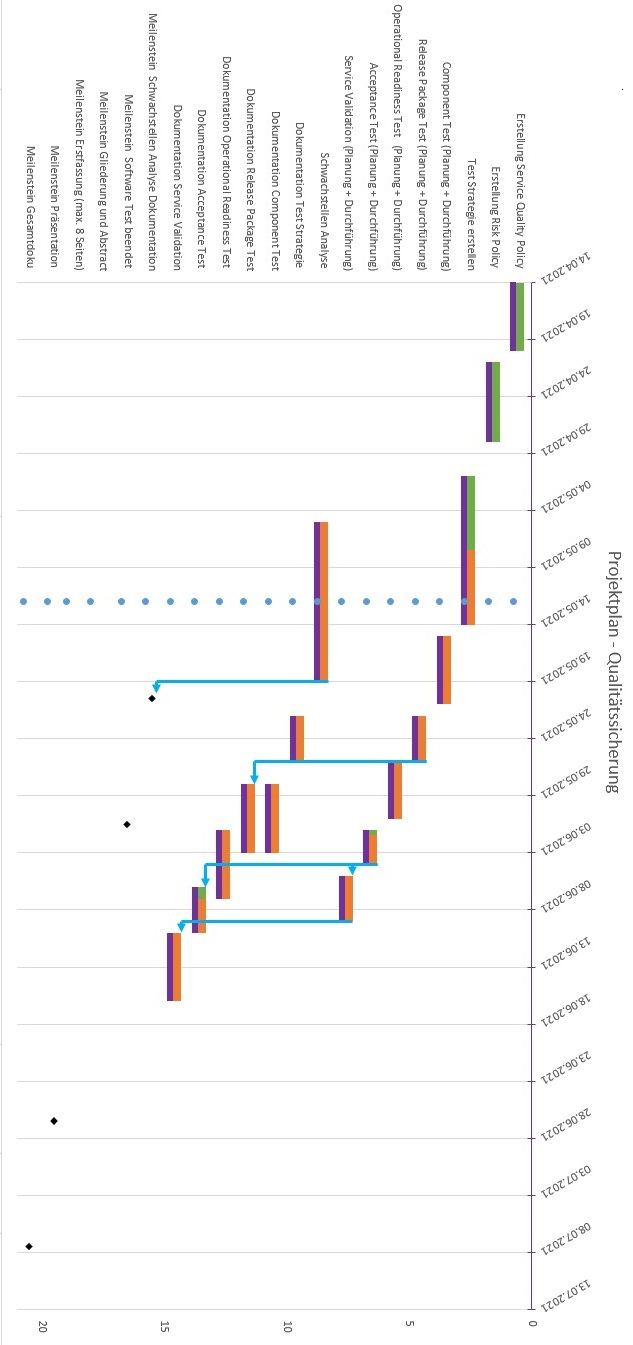
\includegraphics[height=0.95\textheight]{images/Gantt.jpg}
\caption{Projektplan - Qualitätssicherung}
\label{fig:gantt}
\end{figure*}
\FloatBarrier

\subsection{Ablaufplan Analyse Messergebnisse}
\begin{figure*}[thb!]
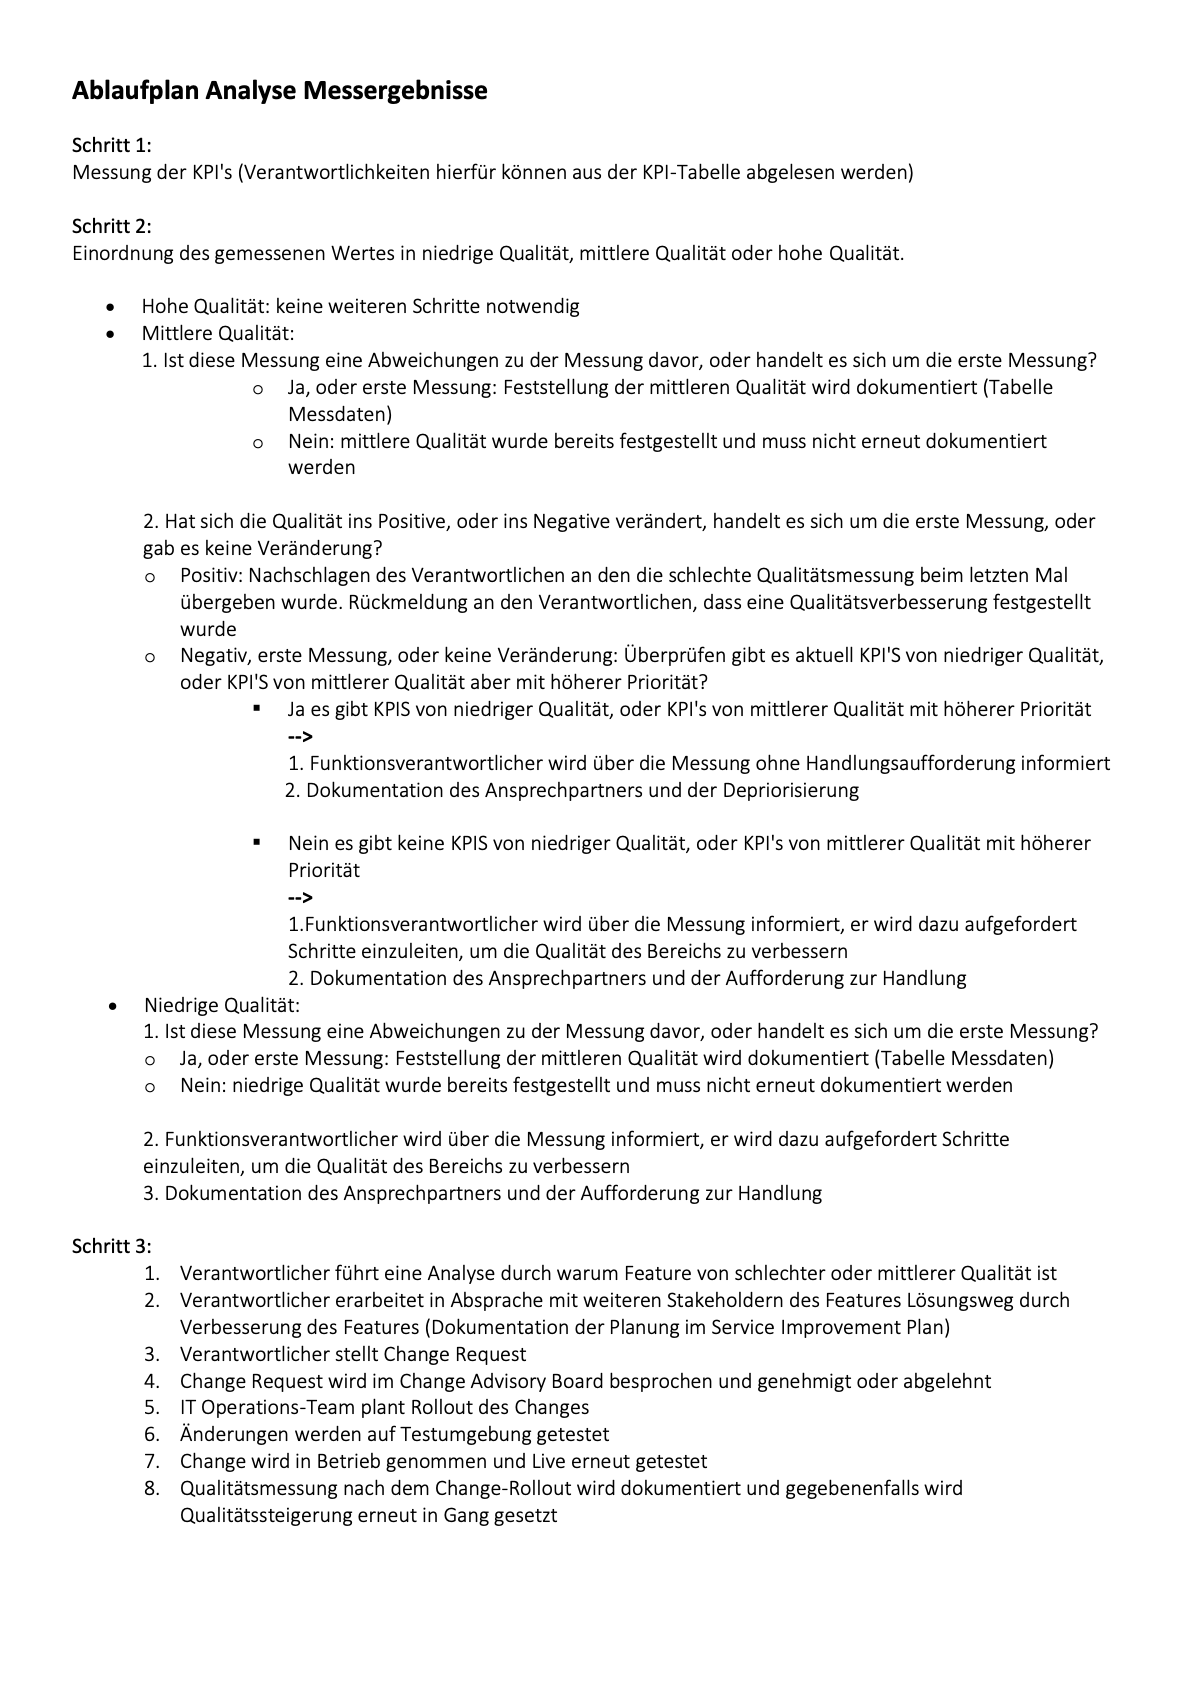
\includegraphics[height=0.95\textheight]{Ablaufplan_Analyse_Messergebnisse.png}
\caption{Ablaufplan Analyse Messergebnisse}
\label{fig:analyseCSI}
\end{figure*}
\FloatBarrier

\end{document}
\endinput
%%
%% End of file `sample-sigconf.tex'.
